\documentclass[tikz]{standalone}
\begin{document}
	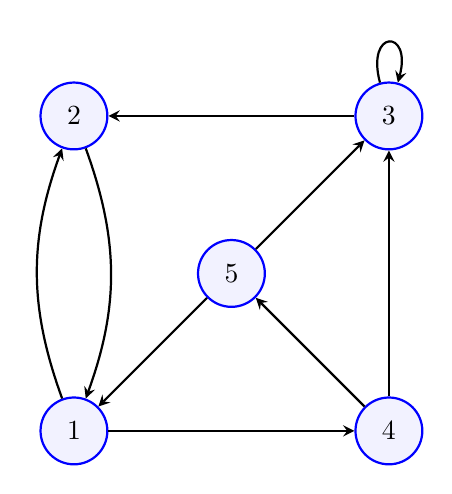
\begin{tikzpicture}[
		inner sep = 2mm,
		->,>= stealth,thick,
		opt/.style={circle,draw=blue,fill=blue!5}
		]
		\node (2) at (0,0) [opt] {$2$};
		\node (3) at (4,0) [opt] {$3$};
		\node (1) at (0,-4) [opt] {$1$};
		\node (4) at (4,-4) [opt] {$4$};
		\node (5) at (2,-2) [opt] {$5$};
		\draw (2) edge [<-] (3) edge [out = -70, in = 70] (1) edge [<-,out = -110, in = 110] (1);
		\draw (4) edge (3) edge [<-] (1) edge (5);
		\draw (5) edge (3) edge (1);
		\draw (3) to[loop above] (3);
	\end{tikzpicture}
\end{document}